%%law inductive

Following is a demonstration of the discretized form from the inductive law (\ref{eq:maxwell_1}). Considering the path integral in a single element edge like Fig.  \ref{fig:FIT_max_integral1},the left side of (\ref{eq:maxwell_1}) can be presented as  (\ref{eq:inductive_left}). 

\begin{figure}[!ht]
\centering
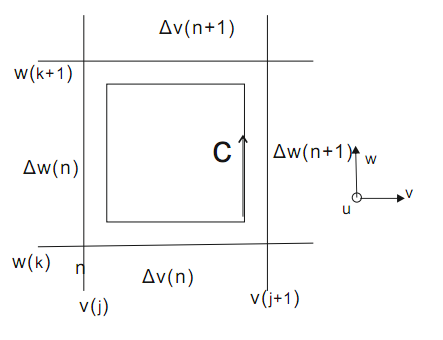
\includegraphics[width=0.45\textwidth]{bilder/FIT_max_integral1}
\caption{ Path integral along edges of one single elemental plane $A_{u}(n)$\cite{ script_FeldSim}}
\label{fig:FIT_max_integral1}
\end{figure}

\begin{figure}[!ht]
\centering
\subfigure[Discrete electric field strength components distribute at edges of grids.]{
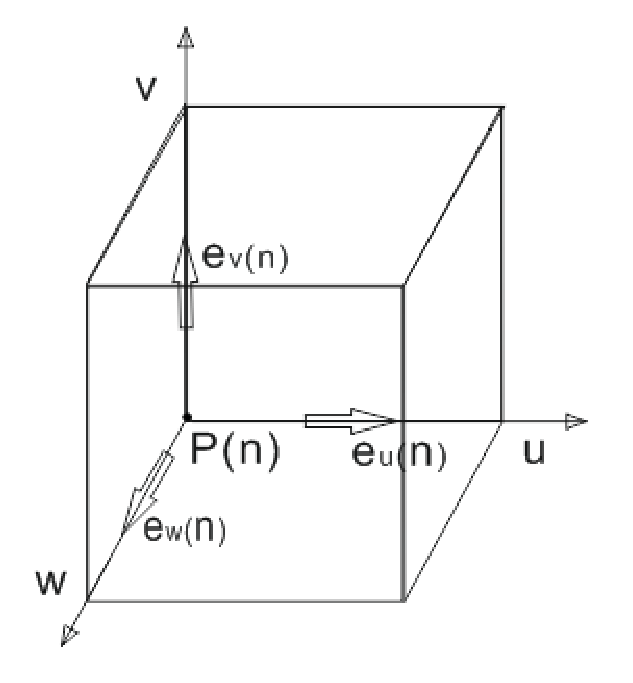
\includegraphics[width=0.4\textwidth]{bilder/FIT_max_integral2}
\label{fig:FIT_max_integral2}
}
\hfill
\subfigure[Discrete magnetic flux density components distribute at planes of grids]{
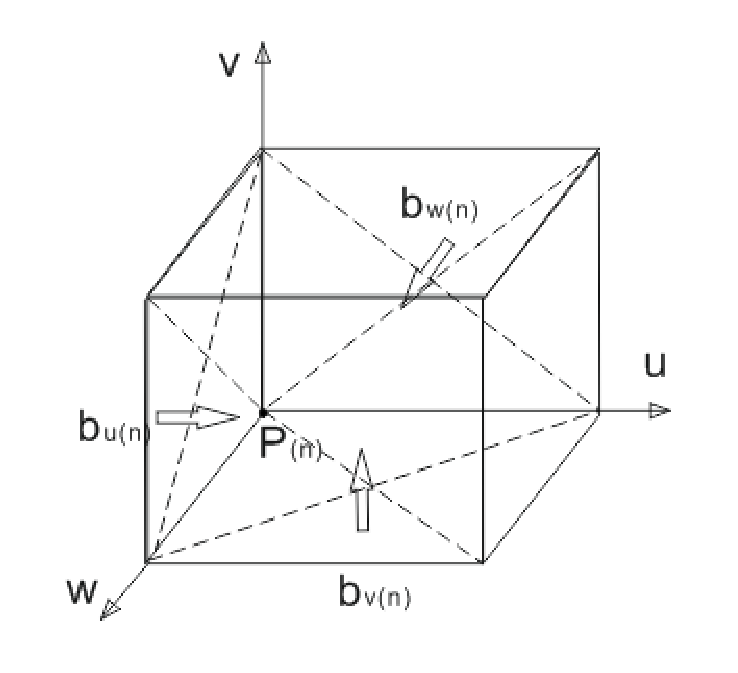
\includegraphics[width=0.4\textwidth]{bilder/FIT_max_integral3}
\label{fig:FIT_max_integral3}
}
\caption{Allocations of components at grids\cite{ script_FeldSim}.}
\end{figure}

\begin{equation}
\int_{C}\vec{E}\cdot d\vec{s}
=\underbrace{\int_{\Delta v(n)}\vec{E}\cdot d\vec{s}}_{\widehat{e}_{v}(n)}
+\underbrace{\int_{\Delta w(n+M_{v})}\vec{E}\cdot d\vec{s}}_{\widehat{e}_{w}(n+M_{v})}
-\underbrace{\int_{\Delta v(n+M_{w})}\vec{E}\cdot d\vec{s}}_{\widehat{e}_{v}(n+M_{w})}
-\underbrace{\int_{\Delta w(n)}\vec{E}\cdot d\vec{s}}_{\widehat{e}_{w}(n)}
\label{eq:inductive_left}
\end{equation}

Where $\widehat{e(n)}$ is so called  electric grid voltage and has the following relation with electric field strength $e(n)$
\begin{equation}
 e_{v}(n)=\frac{\widehat{e}_{v}(n)}{\Delta v(n)}
\label{eq:e_field}
\end{equation}
Meanwhile the right side of (\ref{eq:maxwell_1}) approximates to (\ref{eq:inductive_right})
\begin{equation}
-\iint_{A_{u}(n)}\frac{\partial\vec{B}}{\partial t}\cdot\mathrm{d}\vec{A} 
=-\iint_{A_{u}(n)}\frac{\partial B^{*}_{u}}{\partial t}\cdot\mathrm{d}A
\approx -\frac{\partial}{\partial t}b_{u}(n)A_{u}(n)
\label{eq:inductive_right}
\end{equation}

Where $A_{u}(n)=\Delta v(n)\Delta w(n)$ and $b_{u}(n)$ (Fig.\ref{fig:FIT_max_integral2}) is magnetic flux density
\begin{equation}
 b_{u}(n)=\frac{\widehat{\widehat{b}}_{u}(n)}{\Delta A_{u}(n)}
\label{eq:b_flux_density}
\end{equation}

 and magnetic grid flux $\widehat{\widehat{b}}_{u}(n)$ (\ref{eq:mag_fluxe})
\begin{equation}
\widehat{\widehat{b}}_{u}(n)=\iint_{A_{u}(n)}\vec{B}\cdot\mathrm{d}\vec{A}
\label{eq:mag_fluxe}
\end{equation}

From equations (\ref{eq:inductive_left}-\ref{eq:mag_fluxe}) we obtain the difference form (\ref{eq:inductive_integral}) of the inductive equation at one single elemental plane:
\begin{equation}
\widehat{e}_{v}(n)+\widehat{e}_{w}(n+M_{v})-\widehat{e}_{v}(n+M_{w})-\widehat{e}_{w}(n)=-\frac{\partial}{\partial t}\widehat{\widehat{b}}_{u}(n)
\label{eq:inductive_integral}
\end{equation}
i.e.,
\begin{multline}
\Delta v(n)e_{v}(n)+\Delta w(n+M_{v})e_{w}(n+M_{v})\\
-\Delta v(n+M_{w})e_{v}(n+M_{w})-\Delta w(n)e_{w}(n)=-A_{u}(n)\frac{\partial}{\partial{t}}b_{u}(n) \hspace{5cm}
\label{eq:inductive_sample}
\end{multline}
By merging electric field-strength $e(n)$ and magnetic flux density $b(n)$ of all grids into vectors we obtain:
\begin{equation}
e_{u}:=
\begin{pmatrix}
e_{u}(1)&\\
\vdots&\\
e_{u}(N_{p})&
\end{pmatrix},
e_{v}:=
\begin{pmatrix}
e_{v}(1)&\\
\vdots&\\
e_{v}(N_{p})&
\end{pmatrix},
e_{w}:=
\begin{pmatrix}
e_{w}(1)&\\
\vdots&\\
e_{w}(N_{p})&
\end{pmatrix},
e_{u}:=
\begin{pmatrix}
e_{u}&\\
e_{v}&\\
e_{w}&
\end{pmatrix}.
\label{eq:vector_e_field}
\end{equation}
\begin{equation}
b_{u}:=
\begin{pmatrix}
b_{u}(1)&\\
\vdots&\\
b_{u}(N_{p})&
\end{pmatrix},
b_{v}:=
\begin{pmatrix}
b_{v}(1)&\\
\vdots&\\
b_{v}(N_{p})&
\end{pmatrix},
b_{w}:=
\begin{pmatrix}
b_{w}(1)&\\
\vdots&\\
b_{w}(N_{p})&
\end{pmatrix},
b_{u}:=
\begin{pmatrix}
b_{u}&\\
b_{v}&\\
b_{w}&
\end{pmatrix}.
\label{eq:vector_m_flux_density}
\end{equation}
Expanding the relation (\ref{eq:inductive_sample}) to all grid cells \cite{FIT_discrete_method}\cite{FIT_discrete_electrommagnetism}\cite{FIT_triangular_discretization}\cite{script_FeldSim} we arrive at the discrete form of inductive equation:
\begin{equation}
CD_{s}e=-D_{A}\frac{\partial}{\partial{t}}b
\label{eq:inductive_sample_all}
\end{equation}
Where $D_{s}$ (\ref{eq:Ds_matrix}) is elemental edge matrix,
\begin{equation}
D_{s}=
	\begin{pmatrix}
	\Delta u(1)&&&&&&&&\\
	&\ddots &&&&&&&\\
	&&\Delta u(N_{p})&&&&&&\\
	&&&\Delta v(1)&&&&&\\
	&&&&\ddots &&&&\\
	&&&&&\Delta v(N_{p})&&&\\
	&&&&&&\Delta w(1)&&\\
	&&&&&&&\ddots &\\
	&&&&&&&&\Delta w(N_{p})
	\end{pmatrix}
	\label{eq:Ds_matrix}
\end{equation}
$D_{A}$ (\ref{eq:Da_matrix}) is elemental plane matrix,
\begin{equation}
D_{A}=
	\begin{pmatrix}
	\Delta A_{u}(1)&&&&&&&&\\
	&\ddots &&&&&&&\\
	&&\Delta A_{u}(N_{p})&&&&&&\\
	&&&\Delta A_{v}(1)&&&&&\\
	&&&&\ddots &&&&\\
	&&&&&\Delta A_{v}(N_{p})&&&\\
	&&&&&&\Delta A_{w}(1)&&\\
	&&&&&&&\ddots &\\
	&&&&&&&&\Delta A_{w}(N_{p})
	\end{pmatrix}
	\label{eq:Da_matrix}
\end{equation}
$C$ (\ref{eq:C_matrix}) is \textbf{curl} operator.
\begin{align}
C&=
	\begin{pmatrix}
	&&\quad\vline &\ddots &-1&\quad\vline  &\ddots &+1&\\	
	&0&\quad\vline	& &+1 &\ddots\vline	 &&-1&\ddots\\
	&&\quad\vline	&&&\ddots\vline			 &&&\ddots\\	
	\hline
	\ddots &+1&\quad\vline	&&&\quad\vline	 &\ddots &-1&\\
	&-1 &\ddots\vline	&&0&\quad\vline	&&+1&\ddots\\
	&&\ddots\vline	&&&\quad\vline	&&&\ddots\\
	\hline
	\ddots &-1&\quad\vline &\ddots &+1&\quad\vline	&&&\\
	&+1 &\ddots\vline	&&-1&\ddots\vline	&&0&\\
	&&\ddots\vline		&&&\ddots\vline	&&&
	\end{pmatrix}\nonumber\\
	&=
	\begin{pmatrix}
	0&-P_{w}&P_{v}\\
	P_{w}&0&-P_{u}\\
	-P_{v}&P_{u}&0
	\end{pmatrix}
\label{eq:C_matrix}
\end{align}
Submatrixes $P_{u},P_{v},P_{w}$ are composed of $1,-1,0$ like Fig.\ref{fig:Matrix Px}.\\ 
\begin{figure}[!ht]
\centering
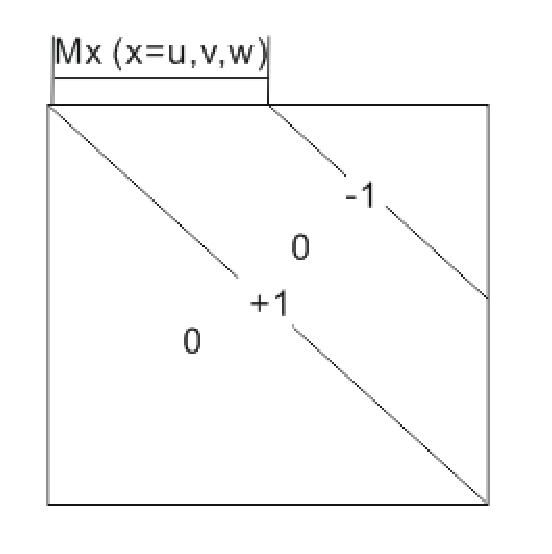
\includegraphics[width=0.5\textwidth]{bilder/P_matrix}
\caption{Matrix $P_{x},(x=u,v,w)$}
\label{fig:Matrix Px}
\end{figure}
Alternative form of the equation(\ref{eq:inductive_sample_all})is given:
\begin{equation}
C\widehat{e}=-\frac{\partial}{\partial{t}}\widehat{\widehat{b}}
\label{eq:inductive_integral_all}
\end{equation}
%\widehat{e}
Where electric voltage $\widehat{e}$ and magnetic flux $\widehat{ \widehat{b}}$ are defined as following:
\begin{equation}
\widehat{e}_{u}:=
\begin{pmatrix}
\widehat{e}_{u}(1)&\\
\vdots&\\
\widehat{e}_{u}(N_{p})&
\end{pmatrix},
\widehat{e}_{v}:=
\begin{pmatrix}
\widehat{e}_{v}(1)&\\
\vdots&\\
\widehat{e}_{v}(N_{p})&
\end{pmatrix},
\widehat{e}_{w}:=
\begin{pmatrix}
\widehat{e}_{w}(1)&\\
\vdots&\\
\widehat{e}_{w}(N_{p})&
\end{pmatrix},
\widehat{e}_{u}:=
\begin{pmatrix}
\widehat{e}_{u}&\\
\widehat{e}_{v}&\\
\widehat{e}_{w}&
\end{pmatrix}.
\label{eq:vector_e_voltage}
\end{equation}
%\widehat{\widehat{b}}
\begin{equation}
\widehat{\widehat{b}}_{u}:=
\begin{pmatrix}
\widehat{\widehat{b}}_{u}(1)&\\
\vdots&\\
\widehat{\widehat{b}}_{u}(N_{p})&
\end{pmatrix},
\widehat{\widehat{b}}_{v}:=
\begin{pmatrix}
\widehat{\widehat{b}}_{v}(1)&\\
\vdots&\\
\widehat{\widehat{b}}_{v}(N_{p})&
\end{pmatrix},
\widehat{\widehat{b}}_{w}:=
\begin{pmatrix}
\widehat{\widehat{b}}_{w}(1)&\\
\vdots&\\
\widehat{\widehat{b}}_{w}(N_{p})&
\end{pmatrix},
\widehat{\widehat{b}}_{u}:=
\begin{pmatrix}
\widehat{\widehat{b}}_{u}&\\
\widehat{\widehat{b}}_{v}&\\
\widehat{\widehat{b}}_{w}&
\end{pmatrix}.
\label{eq:vector_m_flux}
\end{equation}
%divergence equation
\begin{figure}
\centering
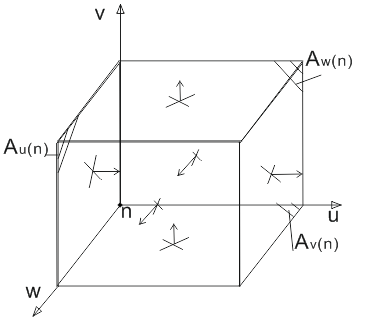
\includegraphics[width=0.5\textwidth]{bilder/divergence_in_grid}
\caption{This figure discribe the allocation of six magnetic facet fluxes in $G$}
\label{fig:divergence_G}
\end{figure}
Analogy the divergence equation(\ref{eq:maxwell_4}) can also be discretized in grid $G$(Fig.\ref{fig:divergence_G}) and can be described in its difference form: 
\begin{equation}
SD_{A}b=0
\label{eq:divergence_sample}
\end{equation}
or
\begin{equation}
S\widehat{\widehat{b}}=0
\label{eq:divergence_integral}
\end{equation}
$S\in \mathbb{R}^{N_{p}\times 3N_{p}}$ represent the discrete divergence matrix, which depends on the grid topology just as the discrete $curl-Matrix$ $C$.
%S
\begin{equation}
S=(P_{u}|P_{v}|P_{w})
\label{eq:S_matrix}
\end{equation}
%Amp\'ere's law
Now considering the discretization of Amp\'ere's law (\ref{eq:maxwell_2}) its magnetic field strengths pass through the elemental plane along the same path with the magnetic flux density (Fig. \ref{fig:divergence_G}). Therefore, a new grid (\textbf{Dual Grid}) like Fig. \ref{fig:dual_grid} is required for this path integral. The second cell $\tilde{G}$ is dual to the primary cell $G$. As primary elements in primary Grid the dual elements are also properly defined in \cite{script_FeldSim}.
\begin{figure}[!ht]
\centering
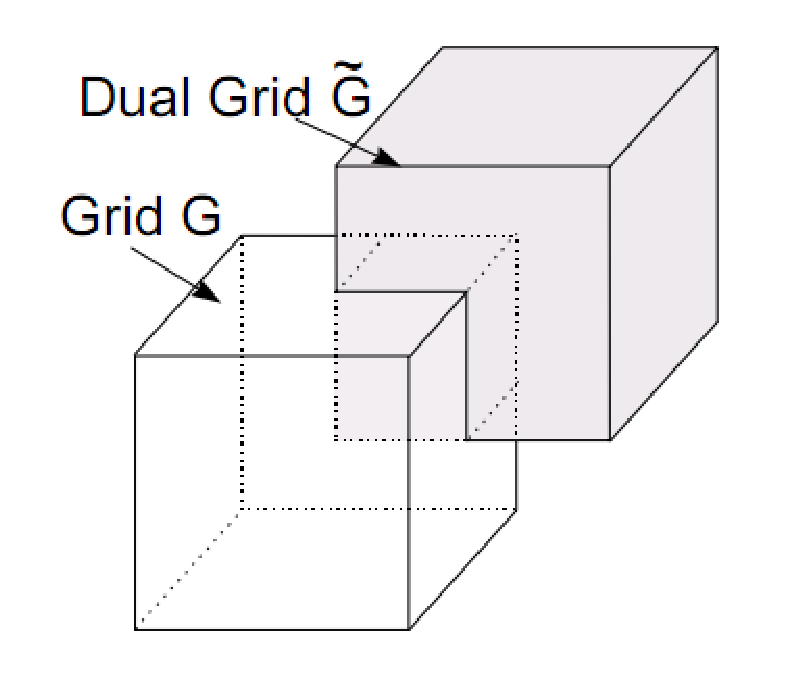
\includegraphics[width=0.5\textwidth]{bilder/dual_grid}
\caption{The allocation of the Primary Grid $G$ and Dual Grid $\tilde{G}$\cite{FIT_discrete_electrommagnetism}.}
\label{fig:dual_grid}
\end{figure}
Like the discretization of Inductive Law Figure. \ref{fig:FIT_max_integral4} and Figure.  \ref{fig:FIT_max_integral5} describe the path integral and surface integral of the equation(\ref{eq:maxwell_2}) in a \textbf{Dual Grid} and lead to the difference equations (\ref{eq:ampere_left_sample}-\ref{eq:ampere_right}).
\begin{figure}
%\centering
	\subfigure[Path Integral of the magnetic flux in dual grid.]{
	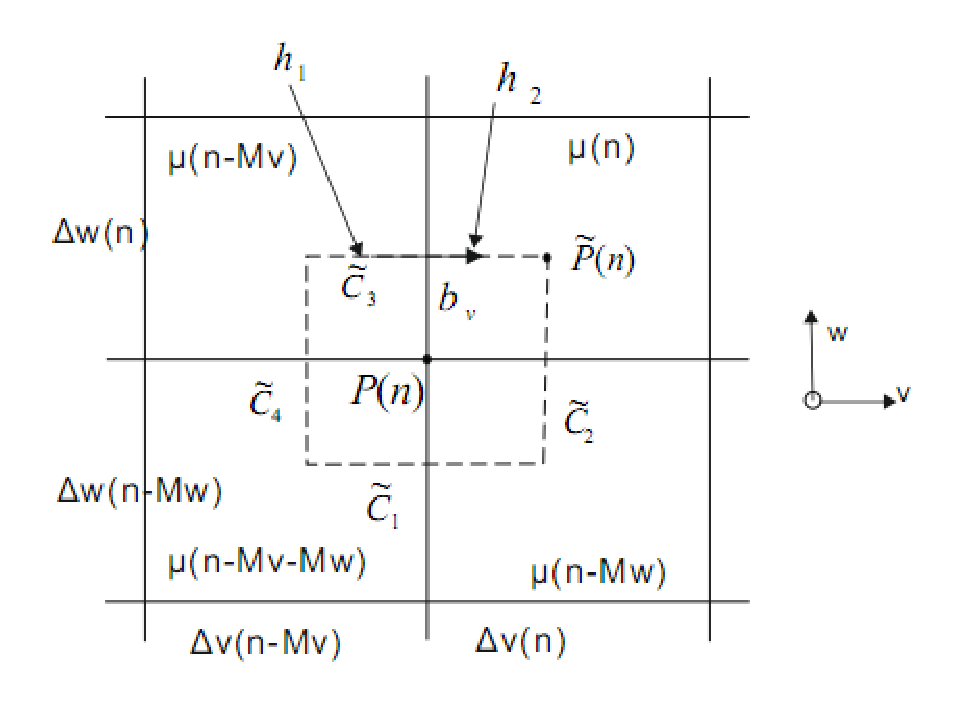
\includegraphics[width=0.5\textwidth]{bilder/FIT_max_integral4}
	\label{fig:FIT_max_integral4}
	}
\hfill
	\subfigure[Surface Integral of the electric flux in dual grid.]{
	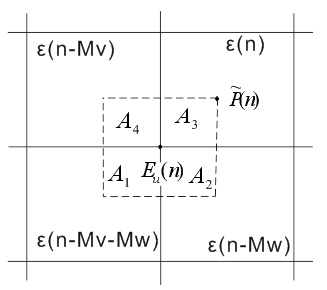
\includegraphics[width=0.4\textwidth]{bilder/FIT_max_integral5}
	\label{fig:FIT_max_integral5}
	}
\caption{Discretization of Amp\'ere's law}
\end{figure}

\begin{equation}
\int_{\tilde{C}}\vec{H}\cdot d\vec{s}=\int_{\tilde{C}}\mu^{-1}\vec{B}\cdot d\vec{s}\approx
\widehat{h}_{v}(n)
+\widehat{h}_{w}(n+M_{v})
-\widehat{h}_{v}(n+M_{w})
-\widehat{h}_{w}(n)
\label{eq:ampere_left_sample}
\end{equation}
\begin{align}
\int\int_{\tilde{A}_{u}}\vec{D}\cdot\mathrm{d}\vec{A}\approx &+e_{u}A_{1}\epsilon_{u}(n-M_{v}-M_{w}) \nonumber\\
&+e_{u}A_{2}\epsilon_{u}(n-M_{w}) \nonumber\\
&+e_{u}A_{3}\epsilon_{u}(n) \nonumber\\
&+e_{u}A_{4}\epsilon_{u}(n-M_{v}) \nonumber\\
&=\bar{\epsilon}_{u}(n)e_{u}\tilde{A}_{u}
\label{eq:ampere_right}
\end{align}
with 
\begin{align}
\widehat{h}_{v}(n)&=h_{1}\cdot\frac{\Delta v(n-M_{v})}{2}+ h_{2}\cdot\frac{\Delta v(n)}{2}\\
h_{1}&=\frac{b_{v}(n)}{\mu (n-M_{v})}\\
h_{2}&=\frac{b_{v}(n)}{\mu (n)}
\label{eq:megnetic_field}
\end{align}

\begin{align}
A_{1}&=\frac{A_{u}(n-M_{v}-M_{w})}{4}\\
A_{2}&=\frac{A_{u}(n-M_{w})}{4}\\
A_{3}&=\frac{A_{u}(n)}{4}\\
A_{4}&=\frac{A_{u}(n-M_{v})}{4}
\end{align}
\begin{align}
\bar{\epsilon}_{x}(n)&:=\frac{\int\int\epsilon\mathrm{d}A}{\int\int\mathrm{d}A}\nonumber\\
&=\frac{1}{4\tilde{A}_{x}(n)}(\epsilon_{x}(n-M_{y}-M_{z})A_{x}(n-M_{y}-M_{z})\nonumber\\
&+\epsilon_{x}(n-M_{z})A_{x}(n-M_{z}) \nonumber\\
&+\epsilon_{x}(n)A_{x}(n) \nonumber\\
&+\epsilon_{x}(n-M_{y})A_{x}(n-M_{y})
\end{align}
$\bar{\epsilon}$ is average dielectric constant. 
The average dielectric matrix is defined:
\begin{equation}
D_{\epsilon}=Diag(\bar{\epsilon}_{u}(1),\ldots,\bar{\epsilon}_{u}(N_{p}),\bar{\epsilon}_{v}(1),\ldots,\bar{\epsilon}_{v}(N_{p}),\bar{\epsilon}_{w}(1),\ldots,\bar{\epsilon}_{w}(N_{p}))
\label{eq:eps_matrix}
\end{equation}
By expanding equations (\ref{eq:ampere_left_sample}-\ref{eq:eps_matrix}) we obtain discretized form(\ref{eq:ampere}) .
\begin{equation}
\tilde{C}\tilde{D}_{s}D_{\mu^{-1}}b=\tilde{D}_{A}(D_{\epsilon}\frac{\mathrm{d}}{\mathrm{dt}}e+D_{\kappa}e+j)
\label{eq:ampere}
\end{equation}
or
\begin{equation}
\tilde{C}\widehat{h}=\frac{\mathrm{d}}{\mathrm{dt}}\widehat{\widehat{d}}+\widehat{\widehat{j}}_{L}+\widehat{\widehat{j}}_{S}
\label{eq:ampere_sample}
\end{equation}
$\tilde{C}$ represents the $curl-operator$ in dual grid.
\begin{equation}
\tilde{C}=
	\begin{pmatrix}
	0&-\tilde{P}_{w}&\tilde{P}_{v}\\
	\tilde{P}_{w}&0&-\tilde{P}_{u}\\
	-\tilde{P}_{v}&\tilde{P}_{u}&0
	\end{pmatrix}
	\label{eq:dual_C_matrix}
\end{equation}
With the help of dual grid cells Gauss' law (\ref{eq:maxwell_3}) in integral form can be discretized\cite{script_FeldSim} as following:
\begin{equation}
\tilde{S}\widehat{\widehat{d}}=q
\label{eq:gausslaw}
\end{equation}
or
\begin{equation}
\tilde{S}\tilde{D}_{A}D_{\epsilon}e=\tilde{D}_{V}\rho_{D}
\label{eq:gausslaw_sample}
\end{equation}
Here $\rho_{D}$ is the vector of the charge density in grid cells.

\begin{equation}
\tilde{S}=(\tilde{P}_{u}|\tilde{P}_{v}|\tilde{P}_{w})=(-P_{u}^{T}|-P_{v}^{T}|\-P_{w}^{T})
\label{eq:dual_S_matrix}
\end{equation}
